\synctex=1
\documentclass[dvipdfmx,10pt, a4j]{jarticle}
%----------------------------------------------------------
%パッケージ読み込み
\usepackage{amsmath}
\usepackage{amssymb}
\usepackage{amsthm} %定理環境の拡張
\usepackage{ascmac}
\usepackage{bm}
\usepackage{cases}
\usepackage{comment} %非表示にするためのコメント
\usepackage{enumerate}
\usepackage{float} %画像をその場に表示.[h]の代わりに[H]
\usepackage{graphicx} % eps 形式の図版取り込みのため
\usepackage{mathrsfs}
\usepackage{url}
\usepackage[dvipdfmx]{hyperref}
\usepackage{color}
\usepackage{mathrsfs}
%----------------------------------------------------------

%----------------------------------------------------------
%命題関係の定義
\theoremstyle{definition}
\newtheorem{definition}{定義}[section]
\newtheorem{theorem}{定理}[section]
\newtheorem{proposition}[theorem]{命題}
\newtheorem{lemma}[theorem]{補題}
\newtheorem{col}[theorem]{系}
\newtheorem{example}{例}[section]
\newtheorem{remark}{注意}[section]
%----------------------------------------------------------

%タイトル・著者===================================================
\title{第10回 数理統計 レポート}
\author{小森 一輝}
%=================================================================

%本文開始=========================================================
\begin{document}

\maketitle

%カウンタ--------------------------------------------------
\setcounter{section}{2}
%\setcounter{subsection}{0}
%\setcounter{subsubsection}{0}
%\setcounter{theorem}{0}

%----------------------------------------------------------定義4.12
\noindent
\textbf{定義 4.12.} n次元連続型確率変数, 同時確率密度関数\\
$n次元確率変数\mathbb{X}に対して, \mathbb{R}^{n}上の非負関数f_{\mathbb{X}}が存在し, 確率分布P_{\mathbb{X}}が$\\
\begin{align*}
    P_X(\textbf{B}) = \int_{\textbf{B}} f_{\mathbb{X}}(x)dx \qquad (\textbf{B} \in \mathscr{B}^{n})\\
\end{align*}
$によって表されるとき, \mathbb{X}は \textbf{n次元連続型確率変数(n dimensional continuous random variable)}と呼ばれ, f_{\mathbb{X}} は$
$\mathbb{X}の \textbf{同時確率密度関数 (join probability density function)}とよばれる.$
$ここで, x=(x_1, x_2, \dots x_n), dx = dx_1dx_2 \cdots dx_n, \int_{\textbf{B}} = \int_{\textbf{B}_1}\int_{\textbf{B}_2}\cdots \int_{\textbf{B}_n}である.$\\
$このとき, \mathbb{X}の同時確率分布関数は,$\\
\begin{align*}
    F_{\mathbb{X}}(x) = \int_{-\infty}^{x_1}\int_{-\infty}^{x_2} \cdots \int_{-\infty}^{x_n} f_{\mathbb{X}}(x)dx\\
\end{align*}
で表される.\\
%---------------以下補足
\begin{itembox}[l]{補足}
    $f_{\mathbb{X}}(x_1, x_2, \dots, x_n) \cdots \mathbb{X}の同時確率密度関数$\\
\end{itembox}\\

%----------------------------------------------------------定義4.13
\noindent
\textbf{定義 4.13.} 周辺確率密度関数\\
$n次元連続確率変数 \mathbb{X} = (X_1, X_2, \dots, X_n)を定義4.4と同様に \textcolor{red}{\mathbb{X} = (\mathbb{X}_{(p)}, (\mathbb{X})_{(q)})}と2つに分ける. このとき, $\\
\begin{align*}
    f_{\mathbb{X}_{(p)}}(x_{(p)}) = \int_{-\infty}^{\infty}\int_{-\infty}^{\infty} \cdots \int_{-\infty}^{\infty} f_{\mathbb{X}}(x)dx_{(q)}\\
\end{align*}
$を \mathbb{X}_{(p)}の\textbf{周辺確率密度関数(marginal probability density function)とよぶ.}$\\

\newpage
%----------------------------------------------------------定義4.14
\noindent
\textbf{定義 4.14.} 条件付き確率密度関数\\
$n次元連続確率変数 \mathbb{X} = (X_1, X_2, \dots, X_n)を定義4.4と同様に\textcolor{red}{\mathbb{X} = (\mathbb{X}_{(p)}, (\mathbb{X})_{(q)})}と2つに分ける. このとき, $\\
\begin{align*}
    f_{\mathbb{X}_{(p)}\mid \mathbb{X}_{(q)}}(x_{(p)}\mid x_{(q)}) = 
    \begin{cases}
        \frac{f_{\mathbb{X}}(x)}{f_{\mathbb{X}_{(q)}}(x_{(q)})} \qquad &(f_{\mathbb{X}_{(q)}}(x_{(q)}) > 0)\\
        0 \qquad &(f_{\mathbb{X}_{(q)}}(x_{(q)}) = 0)
    \end{cases}
\end{align*}

%----------------------------------------------------------例4.6
\noindent
\textbf{例 4.6.} $2次元連続型確率変数(X, Y)の同時確率分布関数\textcolor{red}{F_{X, Y}(x, y)}は,$\\
\begin{align*}
    F_{X, Y}(x, y) = \int_{-\infty}^{x}\int_{-\infty}^{x} f_{X, Y}(s, t)dt\; ds \qquad (f_{X, Y}(s, t) > 0)\\
\end{align*}
$で表され, このときf_{X, Y}(x, y)が同時確率密度関数となる. また, 周辺確率密度関数f_X, f_Y, 条件付き確率密度関数f_{X|Y}は以下で与えられる.$\\
\begin{align*}
    f_X(x) = \int_{-\infty}^{\infty}f_{X, Y}(x, y)dy, \qquad f_Y(y) = \int_{-\infty}^{\infty}f_{X, Y}(x, y)dx\\
    f_{X \mid Y}(x \mid y) = \frac{f_{X, Y}(x, y)}{f_Y(y)}\\
\end{align*}

%---------------以下図
\begin{figure}[htbp]
\begin{center}
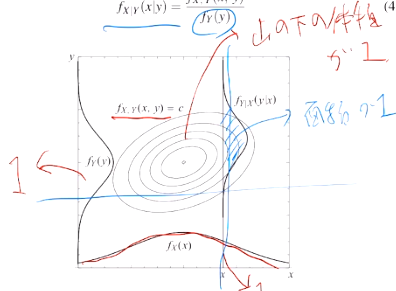
\includegraphics[width=7.0cm]{D_10/img_1.png}
\caption{2次元連続型確率変数の分布}
\end{center}
\end{figure}

%---------------以下図
\begin{figure}[htbp]
\begin{center}
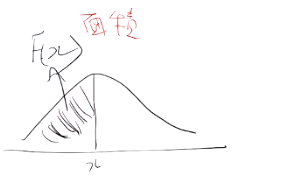
\includegraphics[width=7.0cm]{D_10/img_2.png}
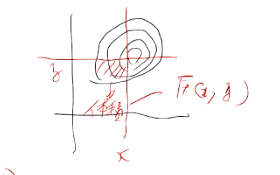
\includegraphics[width=7.0cm]{D_10/img_3.png}
\end{center}
\end{figure}

%---------------以下補足
\begin{itembox}[l]{補足}
    $同時: f_{X, Y}(x, y)$\\
    $周辺: f_{X}(x), f_Y(y)$\\
    $条件付き: f_{X \mid Y}(\textcolor{blue}{x} \mid y), \quad (yが与えられたときのxの\dots) \quad f_{Y \mid X}(y \mid x)$\\
\end{itembox}\\

\newpage
%----------------------------------------------------------定義4.15
\noindent
\textbf{定義 4.15.} n次元確率変数の関数の期待値と分散\\
$n次元確率変数 \mathbb{X}のボレル関数h: \mathbb{R}^{n} \to \mathbb{R} による変数返還h(\mathbb{X})を考える.$
$このとき, h(\mathbb{X})の期待値, 分散を以下で定義する.$\\
\begin{align*}
    &E(h(\mathbb{X})) = 
    \begin{cases}
        \sum^{\infty} \cdots \sum^{\infty}h(x)f_{\mathbb{X}}(x) \qquad &(\mathbb{X}が離散型)\\
        \int_{-\infty}^{\infty} \cdots \int_{-\infty}^{\infty}h(x)f_{\mathbb{X}}(x)dx \qquad &(\mathbb{X}が連続型)\\
    \end{cases}\\
    &V(h(\mathbb{X})) = E\left((h(\mathbb{X})) - E(h(\mathbb{X}))^2 \right)\\
\end{align*}

%---------------以下補足
\begin{itembox}[l]{補足}
    $h(X, Y) = aX + bY \cdots f_{X, Y}$\\
    \begin{align*}
        E(aX + bY) &= \int\int(ax + by)f_{X, Y}(x, y)dxdy\\
        (&= aE(X) + bE(Y))\\
        &= a\int\int xf_{X, Y}(x, y)dxdy + b\int\int yf_{X, Y}(x, y)dxdy\\
        &= a\int\int xf_{X}(x)dx + b\int\int yf_{Y}(y)dy\\
        &= aE(X) + bE(Y)\\
    \end{align*}
\end{itembox}\\
%----------------------------------------------------------例4.7
\noindent
\textbf{例 4.7.} $確率変数 X_1, X_2, \dots, X_n および a_i \in \mathbb{R} (i = 1,2, \dots n)に対して,$\\
\begin{align*}
    E\left(\sum_{i=1}^{n}a_i X_i\right) = \sum_{i=1}^{n}a_i E(X_i)\\
\end{align*}
が成り立つ.\\
$注) x_iは独立とは限らない.$\\
\textcolor{red}{確率変数の和の期待値は, 確率変数の期待値の和}\\
\begin{proof}
    2次元の場合を離散と連続に分ける.\\
    $E(a_1 X_1 + a_2 X_2) = a_1 E(X_1) + a_2 E(X_2)$\\
    \begin{align*}
        E(a_1 X_1 + a_2 X_2) &= \sum_{x_1}\sum_{x_2}(a_1x_1 + a_2x_2)f_{X_1, X_2}(x_1, x_2)\\
        &= \sum_{x_1}\sum_{x_2}a_1x_1f_{X_1, X_2}(x_1, x_2) + \sum_{x_1}\sum_{x_2}a_2x_2f_{X_1, X_2}(x_1, x_2)\\
        &= a_1\sum_{x_1}x_1\textcolor{red}{\sum_{x_2}f_{X_1, X_2}(x_1, x_2)} + a_2\sum_{x_1}x_2\textcolor{red}{\sum_{x_2}f_{X_1, X_2}(x_1, x_2)}\\
        &= a_1\sum_{x_1}x_1\textcolor{red}{f_{X_2}(x_2)} + a_2\sum_{x_1}x_2\textcolor{red}{f_{X_2}(x_2)}\\
        &= a_1 E(X_1) + a_2 E(X_2)\\
    \end{align*}
\end{proof}

%----------------------------------------------------------命題4.8
\noindent
\textbf{命題 4.8.} $確率変数 X_1, X_2, \dots, X_n および a_i \in \mathbb{R} (i = 1,2, \dots n)に対して,$\\
\begin{align*}
    V \left(\sum_{i=1}^{n}a_i X_i \right) &= \sum_{i=1}^{n}\sum_{j=1}^{n}a_i a_j Cov(X_i, X_j)\\
    &= \sum_{i=1}^{n}a_i^2V(X_i) + \sum_{i \neq j}a_i a_j Cov(X_i, X_j)\\
\end{align*}
$が成り立つ.ここで, Cov(X_i, X_j)については, 定義4.16参照.$\\
%---------------以下補足
\begin{itembox}[l]{補足}
    \begin{align*}
        Cov(X_i, X_j) = E((X_i - E(X_i))(X_j - E(X_j)))\\
        Cov(X, Y) &= E_{X, Y}((X_ - E(X))(Y - E(Y)))\\
        &= E_{X, Y}(X Y) - E_{X}(X)E_{Y}(Y)\\
    \end{align*}
\end{itembox}\\
\begin{proof}
    $X_i が独立なら, V(\sum_{i=1}^{n}a_iX_i) = \sum_{i=1}^{n}a_iV(X_i)$\\
    % \begin{align*}
    %     V(\sum a_iX_i) = E((\sum a_i X_i))
    % \end{align*}
    %---------------以下図
    \begin{figure}[htbp]
    \begin{center}
    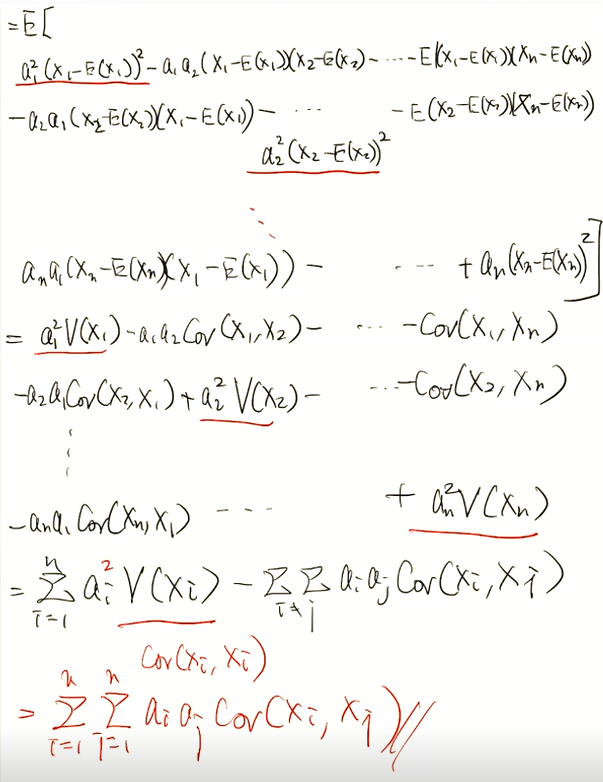
\includegraphics[width=7.0cm]{D_10/img_4.png}
    \caption{}
    \end{center}
    \end{figure}
\end{proof}

%----------------------------------------------------------定理4.9
\noindent
\textbf{定理 4.9.} 確率変数の和の分布\\
$X, Yを離散型または連続型の確率変数とし, それぞれの同時確率関数またが同時確率密度関数をf_{X, Y}で表す.$
$このとき, 確率変数X, Yの和Z = X+Yの確率関数または確率密度関数f_zは,$\\
\begin{align*}
    f_Z(z) = 
    \begin{cases}
        \sum_{i=1}^{\infty}f_{X, Y}(x_i, z - x_i) \qquad &(X, Y が離散型)\\
        \int_{-\infty}^{\infty}f_{X, Y}(x, z - x)dx \qquad &(X, Y が連続型)\\
    \end{cases}\\
\end{align*}
で与えられる.\\

%----------------------------------------------------------定理4.10
\noindent
\textbf{定理 4.10.} 確率変数の積と商の分布\\
$X, Yを連続型の確率変数とし, それぞれおの同時確率密度関数をf_{X, Y}で表す.$
$このとき, 確率変数X. Y の積 Z_1 = XY, 商Z_2 = X/Y の確率密度関数f_{Z_1}, f_{Z_2}は,$\\
それぞれ,\\
\begin{align*}
    &f_{Z_1(z_1)} &= \int_{-\infty}^{\infty}f_{X, Y}\left(x, \frac{z_1}{x}\right)\frac{1}{|x|}dx &= \int_{-\infty}^{\infty}f_{X, Y}\left(\frac{z_1}{y}, y \right)\frac{1}{|y|}dy\\
    &f_{Z_2(z_2)} &= \int_{-\infty}^{\infty}f_{X, Y}\left(x, \frac{x}{z_2}\right)\frac{|x|}{z_2^2}dx &= \int_{-\infty}^{\infty}f_{X, Y}\left(z_2y, y \right)|y|dy\\
\end{align*}
で与えられる.\\

\noindent
{\LARGE 4.3 2次元確率変数の特性値}\\

%----------------------------------------------------------定理4.16
\noindent
\textbf{定理 4.16.} 2次元確率変数(X, Y)の積率\\
$2次元確率変数(X, Y)の原点まわりの i \neq j 次積率 \mu_{ij}^{\prime}および, 平均まわりのi \neq j 次積率\mu_{ij}をそれぞれ以下のように定める.$\\
\begin{align*}
    \mu_{ij}^{\prime} = E(X^{i}Y^{j}), \qquad \mu_{ij} = E((X - E(X))^{i}(Y - E(Y))^{j})\\
\end{align*}
$特に, \mu_{11} を X と Y の \textbf{共分散(covariance)}とよび, Cov(X, Y)と記す.$\\

%----------------------------------------------------------命題4.11
\noindent
\textbf{命題 4.11.} 共分散の性質\\
$共分散Cov(X, Y)について, 以下が成り立つ.$\\
\begin{enumerate}[i)]
    \item $Cov(X, Y) = Cov(Y, X)$\\
    \item $Cov(X, X) = V(X),\quad Cov(Y, Y) = V(Y)$\\
    \item $Cov(X, Y) = E(XY) - E(X)E(Y)$\\
    \item $(Cov(X, Y))^2 \leq V(X)V(Y)$\\
\end{enumerate}


\end{document}
%本文ここまで=========================================================
